\documentclass{VUMIFInfKursinis}
\usepackage{algorithmicx}
\usepackage{algorithm}
\usepackage{algpseudocode}
\usepackage{amsfonts}
\usepackage{amsmath}
\usepackage{bm}
\usepackage{caption}
\usepackage{color}
\usepackage{float}
\usepackage{graphicx}
% \usepackage{hyperref}  % Nuorodų aktyvavimas
\usepackage{listings}
\usepackage{subfig}
\usepackage{url}
\usepackage{wrapfig}


% Titulinio aprašas
\university{Vilniaus universitetas}
\faculty{Matematikos ir informatikos fakultetas}
\department{Informatikos katedra}
\papertype{Kursinis darbas}
\title{Rizikų valdymo proceso modeliavimas}
\titleineng{Modeling of Risk Management Process}
\status{X kurso Y grupės studentas}
\author{Vardenis Pavardenis}
% \secondauthor{Vardonis Pavardonis}   % Pridėti antrą autorių
\supervisor{prof. habil. dr. Vardaitis Pavardaitis}
\date{Vilnius \\ \the\year}

% Nustatymai
% \setmainfont{Palemonas}   % Pakeisti teksto šriftą į Palemonas (turi būti įdiegtas sistemoje)
\bibliography{bibliografija} 

\begin{document}
\maketitle

\tableofcontents

\sectionnonum{Sąvokų apibrėžimai}
Sutartinių ženklų, simbolių, vienetų ir terminų sutrumpinimų sąrašas (jeigu
ženklų, simbolių, vienetų ir terminų bendras skaičius didesnis nei 10 ir
kiekvienas iš jų tekste kartojasi daugiau nei 3 kartus).

\sectionnonum{Įvadas}
Įvade apibūdinamas darbo tikslas, temos aktualumas ir siekiami rezultatai.

\section{Pagrindinė tiriamoji dalis}
Pagrindinėje tiriamojoje dalyje aptariama ir pagrindžiama tyrimo metodika;
pagal atitinkamas darbo dalis, nuosekliai, panaudojant lyginamosios analizės,
klasifikacijos, sisteminimo metodus bei apibendrinimus, dėstoma sukaupta ir
išanalizuota medžiaga. 

\subsection{Poskyris}
Citavimo pavyzdžiai: cituojamas vienas šaltinis \cite{PvzStraipsnLt}; cituojami
keli šaltiniai \cite{PvzStraipsnEn, PvzKonfLt, PvzKonfEn, PvzKnygLt, PvzKnygEn,
PvzElPubLt, PvzElPubEn, PvzMagistrLt, PvzPhdEn}.

\subsubsection{Skirsnis}
\subsubsubsection{Straipsnis}
\subsubsection{Skirsnis}
\section{Skyrius}
\subsection{Poskyris}
\subsection{Poskyris}

\sectionnonum{Išvados}
Išvadose ir pasiūlymuose, nekartojant atskirų dalių apibendrinimų,
suformuluojamos svarbiausios darbo išvados, rekomendacijos bei pasiūlymai.

\printbibliography[heading=bibintoc] % Literatūros šaltiniai aprašomi
% bibliografija.bib faile. Šaltinių sąraše nurodoma panaudota literatūra,
% kitokie šaltiniai. Abėcėlės tvarka išdėstoma tik darbe panaudotų (cituotų,
% perfrazuotų ar bent paminėtų) mokslo leidinių, kitokių publikacijų
% bibliografiniai aprašai (šiuo punktu pasirūpina LaTeX). Aprašai pateikiami
% netransliteruoti.

\appendix  % Priedai
% Prieduose gali būti pateikiama pagalbinė, ypač darbo autoriaus savarankiškai
% parengta, medžiaga. Savarankiški priedai gali būti pateikiami kompiuterio
% diskelyje ar kompaktiniame diske. Priedai taip pat vadinami ir numeruojami.
% Tekstas su priedais siejamas nuorodomis (pvz.: \ref{img:mlp}).

\section{Niauroninio tinklo struktūra}
\begin{figure}[H]
    \centering
    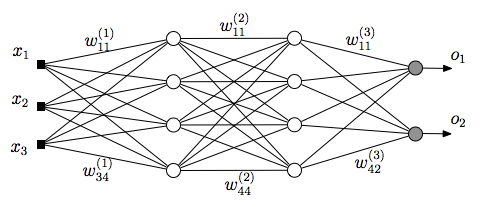
\includegraphics[scale=0.5]{img/MLP}
    \caption{Paveikslėlio pavyzdys}
    \label{img:mlp}
\end{figure}


\section{Eksperimentinio palyginimo rezultatai}
% tablesgenerator.com - converts calculators (e.g. excel) tables to LaTeX
\begin{table}[H]\footnotesize
  \centering
  \caption{Lentelės pavyzdys.}
  {\begin{tabular}{|l|c|c|} \hline
    Algoritmas & $\bar{x}$ & $\sigma^{2}$ \\
    \hline
    Algoritmas A  & 1.6335    & 0.5584       \\
    Algoritmas B  & 1.7395    & 0.5647       \\
    \hline
  \end{tabular}}
  \label{tab:table example}
\end{table}

\end{document}
